\documentclass[aspectratio=169,13pt,fleqn,t] {beamer}
%
% Choose how your presentation looks.
%
% For more themes, color themes and font themes, see:
% http://deic.uab.es/~iblanes/beamer_gallery/index_by_theme.html
%
\mode<presentation>
{
	\usetheme{Madrid}      % 整体主题
	\usecolortheme{beaver} % 配色主题（棕红系）
	\usefonttheme{serif}   % 全局衬线字体（正文宋体类）
	\setbeamertemplate{items}[default] % 【items父模板】控制 itemize+enumerate 符号
%	\setbeamertemplate{items}{\Large\beamertemplateballitem}
	\setbeamertemplate{sections/subsections in toc}[ball] % 目录里章节用圆圈标记
	
	%  \setbeamertemplate{navigation symbols}{} % 取消注释可隐藏底部导航小图标
	\setbeamertemplate{caption}[numbered] % 图/表标题带编号：图1、表1
	\setbeamertemplate{theorems}[numbered]
}

\usepackage[UTF8,linespread=1.2]{ctex}
\usepackage{wrapfig}
\usepackage{caption}
\usepackage{tcolorbox}
\tcbuselibrary{skins}
\captionsetup[figure]{name=图,labelsep=period}

\usepackage{calligra}
%如果你需要在 LaTeX 文档中插入具有书法/手写风格的英文（或特定字符）文本，可以使用这个宏包，通过 \calligra 或 \textcalligra{} 来实现。使用 {\Huge\calligra Thanks!} 就能利用这个宏包输出优雅的书法体“Thanks!”。

\usepackage{xcolor}
\definecolor{xy_blue}{cmyk}{0.6,0.35,0.0,0.4}
\definecolor{xy_orange}{cmyk}{0.0,0.7,1.0,0.0}
\definecolor{xy_green}{cmyk}{0.2,0.0,1.0,0.15}
\xdefinecolor{xy_gold}{RGB}{135,103,79}
\xdefinecolor{xy2_gold}{cmyk}{0,0.35,0.75,0.05}

\setbeamercolor{section number projected}{fg=red,bg=red!20}%控制球的颜色
\setbeamercolor{subsection number projected}{fg=blue,bg=blue!40}
\setbeamercolor{item}{fg=xy_gold} %设置列表项颜色

\usepackage{amsthm}
\newtheorem{peroration}{结论：}
\newtheorem*{exploration}{探究：}
\newtheorem*{prooft}{证明：}
\newtheorem*{solve}{解:} 
\newtheorem{instance}{例}   % 解：独立计数器
     

% 配色（你前面需要的，每个环境单独颜色）
\setbeamercolor{theorem}{fg=black,bg=blue!10}
\setbeamercolor{solution}{fg=black,bg=green!10}

\BeforeBeginEnvironment{peroration}{%结论： 
	\setbeamercolor{block title}{bg=xy_green,fg=white}
	\setbeamercolor{block body}{bg=xy_green!10}
}
\AfterEndEnvironment{peroration}{
	\setbeamercolor{block title}{bg=xy_blue,fg=white}
	\setbeamercolor{block body}{bg=xy_blue!10}
}
\BeforeBeginEnvironment{exploration}{%探究
	\setbeamercolor{block title}{bg=xy_orange,fg=white}
	\setbeamercolor{block body}{bg=xy_orange!10}
}
\AfterEndEnvironment{peroration}{
	\setbeamercolor{block title}{bg=xy_blue,fg=white}
	\setbeamercolor{block body}{bg=xy_blue!10}
}
\BeforeBeginEnvironment{solution}{%解
	\begingroup
	\setbeamercolor{block title}{bg=xy_green,fg=white}
	\setbeamercolor{block body}{bg=xy_green!10}
}
\AfterEndEnvironment{solution}{
	\endgroup
}
\BeforeBeginEnvironment{prooft}{%证明
	\setbeamercolor{block title}{bg=xy_green,fg=white}
	\setbeamercolor{block body}{bg=xy_green!10}
}
\AfterEndEnvironment{prooft}{
	\setbeamercolor{block title}{bg=xy_green,fg=white}
	\setbeamercolor{block body}{bg=xy_green!10}
}
\BeforeBeginEnvironment{solve}{%解：
	\setbeamercolor{block title}{bg=xy_orange!60,fg=white}
	\setbeamercolor{block body}{bg=xy_orange!10}
}
\AfterEndEnvironment{solve}{%解：
	\setbeamercolor{block title}{bg=xy_orange!60,fg=white}
	\setbeamercolor{block body}{bg=xy_orange!10}
}
   
\BeforeBeginEnvironment{instance}{% 例子
	\begingroup
   	\setbeamercolor{block title}{bg=xy_gold!40,fg=black}
   	\setbeamercolor{block body}{bg=xy_gold!10}
   }
\AfterEndEnvironment{instance}{
	\endgroup
   }     
   
\renewcommand{\thefigure}{\arabic{figure}}

\title[2.2基本不等式]{2.2~~基本不等式(教材习题答案解析)}
\author[好好学习，努力向上]{}
\institute{}
\date{2026.9.29}


\AtBeginSection[]
{
  \begin{frame}<beamer>
    \frametitle{本节主要内容}
    \tableofcontents[currentsection,currentsubsection]
  \end{frame}
}


\begin{document}
\begin{frame}{}
	\titlepage
\end{frame}


%1.
\begin{frame}
	\begin{enumerate}[1.]
		\item 用 \(20\text{ cm}\) 长的铁丝折成一个面积最大的矩形，应当怎样折？
	\end{enumerate}

	\leftskip=2em
	\begin{minipage}{0.8\textwidth}
	
	\begin{solve}
		设矩形的相邻两条边的长分别为 $x\ \mathrm{cm}$，$y\ \mathrm{cm}$，
		
		由周长为为 $2(x+y)\ = 20$得$x+y=10$。于是矩形的面积
		\[
		S=xy \leqslant (\frac{x+y}{2})^2 =25
		\]
		当且仅当$x=y=5$时取等号，所以当把矩形做成边长为$5\mathrm{cm}$的正方形时时面积最大。		
	\end{solve}
	\end{minipage}

\end{frame}

%2.
\begin{frame}
	\begin{enumerate}[2.]
		\item 用一段长为 \(30\text{ m}\) 的篱笆围成一个一边靠墙的矩形菜园，墙长 \(18\text{ m}\)。当这个矩形的边长为多少时，菜园的面积最大？最大面积是多少？
	\end{enumerate}
	
	\leftskip=2em
	\begin{minipage}{0.8\textwidth}
		
		\begin{solve}
			设矩形平行于墙的一边长为 $x\ \mathrm{m}$，另两边均为$y\ \mathrm{m}$，
			
			依题意得，$x+2y=30$，$0<x \leqslant 18$，
			
			于是矩形菜园的面积
			\[
			S=xy =\frac{1}{2}\cdot x\cdot 2y \leqslant\frac{1}{2} \left(\frac{x+2y}{2}\right)^2 =\frac{225}{2}
			\]
			当且仅当$x=2y=15$时取等号，所以当把矩形做成平行于墙的一边长为$15\mathrm{m}$，另两边长都为$\frac{15}{2}\mathrm{m}$时矩形菜园的面积最大。		
		\end{solve}
	\end{minipage}
	
\end{frame}


%3.
\begin{frame}
	\begin{enumerate}[3.]
		\item 做一个体积为 \(32\text{ m}^3\)，高为 \(2\text{ m}\) 的长方体纸盒，当底面的边长取什么值时，用纸最少？
	\end{enumerate}
	
	\leftskip=2em
	\begin{minipage}{0.8\textwidth}
		
		\begin{solve}
			设底面矩形的两边长分别为 $x\ \mathrm{m}$，$y\ \mathrm{m}$，
			
			依题意得，$xy=\frac{32}{2} = 16$，长方体的表面积	
			\begin{align*}
			S_{\text{表}}&=2xy + 2(2x+2y) =32 + 4 (x+y)\\
			&\geqslant 32 + 4\sqrt{xy} = 32+4\times 4 \\
			&=48 
			\end{align*}
			当且仅当$x=y=4$时取等号，所以当把底面边长做成边长为$4\mathrm{m}$的正方形时用纸最少。
		\end{solve}
	\end{minipage}
	
\end{frame}

%4.
\begin{frame}
	\begin{enumerate}[4.]
		\item 已知一个矩形的周长为 \(36\text{ cm}\)，矩形绕它的一条边旋转形成一个圆柱。当矩形的边长为多少时，旋转形成的圆柱的侧面积最大？
	\end{enumerate}
	
	\leftskip=2em
	\begin{minipage}{0.8\textwidth}
		
		\begin{solve}
			设矩形通过绕一边旋转的边长为 $x\ \mathrm{cm}$，另一边长为$y\ \mathrm{cm}$，
			
			依题意得，$2(x+y)=36$，所以$x+y=18$，于是圆柱的侧面积
			\begin{align*}
				S_{\text{侧}}&=2\pi \cdot xy \\
				&\geqslant 2\pi \left(\frac{x+y}{2} \right)^2= 2\pi \times 81 \\
				&=162\pi 
			\end{align*}
			当且仅当$x=y=9$时取等号，所以当矩形相邻两条边长均为$6\mathrm{cm}$时，圆柱的侧面积最大。
		\end{solve}
	\end{minipage}
	
\end{frame}

%5.
\begin{frame}
	\begin{enumerate}[5.]
		 \item 某公司建造一间背面靠墙的房屋，地面面积为 \(48\text{ m}^2\)，房屋正面每平方米的造价为 \(1200\) 元，房屋侧面每平方米的造价为 \(800\) 元，屋顶的造价为 \(5800\) 元。如果墙高为 \(3\text{ m}\)，且不计房屋背面和地面的费用，那么怎样设计房屋能使总造价最低？最低总造价是多少？
	\end{enumerate}
	
	\leftskip=2em
	\begin{minipage}{0.8\textwidth}
		
		\begin{solve}
		设房屋地面相邻两边边长分别为 \(x\;\mathrm{ m}\)，\(y\;\mathrm{ m}\)，总造价为 \(z\) 元。
		
		因为 \(xy = 48\)，所以
		\vspace{-1ex}	
		\begin{align*}
			z &= 3600y + 4800x + 5800 = \frac{48 \times 3600}{x} + 4800x + 5800\\
			&\geqslant 2\sqrt{48 \times 3600 \times 4800} + 5800 \\
			&= 2 \times 4 \times 3600 + 5800 = 34600,
		\end{align*}
		
		\vspace{-1em}
		  当 \(x = 6\) 时，上式取等号。所以当房屋地面相邻两边边长分别建成 $6 \mathrm{m}$ 和 $8\mathrm{m}$ 时，造价最低，最低总造价为 $34600$ 元。
		\end{solve}
	\end{minipage}
	
\end{frame}

%6.
\begin{frame}
	\begin{enumerate}[6.]
		\item 已知 \(x, y, z\) 都是正数，求证：\((x+y)(y+z)(z+x) \geqslant 8xyz\)。
	\end{enumerate}
	
	\leftskip=2em
	\begin{minipage}{0.8\textwidth}
		
		\begin{prooft}
			因为\(x > 0, y > 0, z > 0\)，
			
			所以
			\[x + y \geqslant 2\sqrt{xy},\quad y + z \geqslant 2\sqrt{yz},\quad x + z \geqslant 2\sqrt{xz},\]
			从而 
			\[(x+y)(y+z)(z+x) \geqslant 8\sqrt{xy} \cdot \sqrt{yz} \cdot \sqrt{xz} = 8xyz.\]
		\end{prooft}
	\end{minipage}
	
\end{frame}

%7.
\begin{frame}
	\begin{enumerate}[7.]
		\item 已知 \(x > 0\)，求证：\(2 - 3x - \frac{4}{x}\) 的最大值是 \(2 - 4\sqrt{3}\)。
	\end{enumerate}
	
	\leftskip=2em
	\begin{minipage}{0.8\textwidth}
		
		\begin{prooft}
			 因为 \(x > 0\)，
			 所以 \[3x + \frac{4}{x} \geqslant 2\sqrt{3x \cdot \frac{4}{x}} = 4\sqrt{3},\]
			 当且仅当 \(3x = \frac{4}{x}\)，解得$x=\frac{2\sqrt{3}}{3}$ 时，上式等号成立。
			 
			 因此，
			 \[
			 2 - 3x - \frac{4}{x} = 2 - \left(3x + \frac{4}{x}\right) \leqslant 2 - 4\sqrt{3}.
			 \]
			 即\(2 - 3x - \frac{4}{x}\) 的最大值是 \(2 - 4\sqrt{3}\)。
		\end{prooft}
	\end{minipage}
	
\end{frame}


%8.
\begin{frame}
	\begin{enumerate}[8.]
		\item 一家货物公司计划租地建造仓库储存货物，经过市场调查了解到下列信息：每月土地占地费 \(y_1\)（单位：万元）与仓库到车站的距离 \(x\)（单位：\(\text{km}\)）成反比，每月库存货物费 \(y_2\)（单位：万元）与 \(x\) 成正比；若在距离车站 \(10\text{ km}\) 处建仓库，则 \(y_1\) 和 \(y_2\) 分别为 \(2\) 万元和 \(8\) 万元。这家公司应该把仓库建在距离车站多少千米处，才能使两项费用之和最小？
	\end{enumerate}
	
	\leftskip=2em
	\begin{minipage}{0.9\textwidth}
		
		\begin{solve}
			设 \(y_1 = \frac{k_1}{x}\)，\(y_2 = k_2x\)。由题意，当$x=10$时，$y_1=2$，$y_2=8$，所以$k_1 = 2\times 10 = 20$，$k_2= \frac{8}{10} = 0.8$。
			
			所以
			 \[y_1 + y_2 =\frac{20}{x} + 0.8x \geqslant 2\sqrt{\frac{20}{x}\cdot 0.8x} = 2\sqrt{16} = 8,\]
			 当 $\frac{20}{x} = 0.8x$解得\(x = 5\) 时上式取等号，所以，当把仓库建在距离车站 $5\mathrm{km}$ 处时，两项费用之和最小。
		\end{solve}
	\end{minipage}
	
\end{frame}

%9.
\begin{frame}
	\begin{enumerate}[9.]
		\item 一家商店使用一架两臂不等长的天平称黄金。一位顾客到店里购买 \(10\text{ g}\) 黄金，售货员先将 \(5\text{ g}\) 的砝码放在天平左盘中，取出一些黄金放在天平右盘中使天平平衡；再将 \(5\text{ g}\) 的砝码放在天平右盘中，再取出一些黄金放在天平左盘中使天平平衡；最后将两次称得的黄金交给顾客。你认为顾客购得的黄金是小于 \(10\text{ g}\)，等于 \(10\text{ g}\)，还是大于 \(10\text{ g}\)？为什么？
	\end{enumerate}
	
	\leftskip=2em\vspace{-1ex}
	\begin{minipage}{0.9\textwidth}
		
		\begin{solve}
			设天平的左臂长为 \(a\;\mathrm{ cm}\)，右臂长为 \(b\;\mathrm{ cm}\)，不妨设 \(a > b\)，放在左盘中的黄金为 \(x \;\mathrm{ g}\)，放在右盘中的黄金为 \(y\;\mathrm{ g}\)。
			
			则由天平的平衡条件可得 \(bx = 5a\)，\(ay = 5b\)，即 \(x = \frac{5a}{b}\)，\(y = \frac{5b}{a}\)，
			
			所以，
			\[
			x + y \geqslant 2\sqrt{xy} = 10.
			\]
			因此，顾客购得的黄金大于 $10 \;\mathrm{g}$。
		\end{solve}
	\end{minipage}
\end{frame}

%10.
\begin{frame}
	\begin{enumerate}[10.]
	\item 设矩形 \(ABCD\)（\(AB > AD\)）的周长为 \(24\text{ cm}\)，把 \(\triangle ABC\) 沿 \(AC\) 向 \(\triangle ADC\) 折叠，\(AB\) 折过去后交 \(DC\) 于点 \(P\)。设 \(AB = x\text{ cm}\)，求 \(\triangle ADP\) 的最大面积及相应 \(x\) 的值。
	\end{enumerate}
	
	\vspace{-1ex}\leftskip=2em
	\begin{minipage}{0.9\textwidth}
		\begin{solve}			
			\begin{wrapfigure}{r}{0.32\textwidth}
			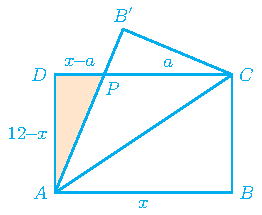
\includegraphics{Figures/rectangle.pdf}
			\end{wrapfigure}
			
			设 \(AB = x\)，则 \(AD = 12 - x\)。设 \(PC = a\)，
			
			则 \(DP = x - a\)，$AP = PC = a$。
			
			所以在三角形$ADP$中，由勾股定理，
			
			\((12-x)^2 + (x-a)^2 = a^2\)，
			
			可得 \(a = \frac{x^2 - 12x + 72}{x}\)，\(DP = x - a = \frac{12x - 72}{x}\)。
			
			所以 \(\triangle ADP\) 的面积\vspace{-1ex}
			 \[
			 S = \frac{1}{2}(12-x)\frac{12x-72}{x} = 6\left[-\left(x + \frac{72}{x}\right) + 18\right].
			 \]
			 
			\vspace{-1ex}
			所以 \(S \leqslant 6\left[-2\sqrt{72} + 18\right] = 108 - 72\sqrt{2}\)，
			
			即 \(x = 6\sqrt{2}\mathrm{ cm}\) 时，\(\triangle ADP\) 的面积最大，最大面积是 \((108 - 72\sqrt{2})\mathrm{ cm}^2\)。		
		\end{solve}
	\end{minipage}
\end{frame}
\begin{frame}[c]
	\begin{center}
		{\Huge\calligra Thanks!}
	\end{center}
\end{frame}

\end{document}
